\documentclass[tikz,border=6pt]{standalone}
% Shared visual language for the book's standalone vector figures.
% Keep this file compatible with the TeX Live version used by LyX.
\usepackage{amsmath,amssymb}
\usepackage{array,booktabs}
\usepackage{pgfplots}
\usepackage{pgfplotstable}
\usetikzlibrary{arrows.meta,calc,positioning}
\pgfplotsset{compat=1.17}

\definecolor{BookBlue}{HTML}{0072B2}
\definecolor{BookOrange}{HTML}{D55E00}
\definecolor{BookGreen}{HTML}{009E73}
\definecolor{BookGray}{HTML}{666666}
\definecolor{BookLightGray}{HTML}{D9D9D9}

\pgfplotsset{
  book axis/.style={
    axis line style={black!75,line width=0.55pt},
    tick style={black!75,line width=0.45pt},
    tick label style={font=\small},
    label style={font=\small},
    legend style={
      font=\small,
      draw=none,
      fill=none,
      cells={anchor=west},
    },
    grid style={BookLightGray,line width=0.35pt},
    major grid style={BookLightGray,line width=0.35pt},
  },
}

\begin{document}
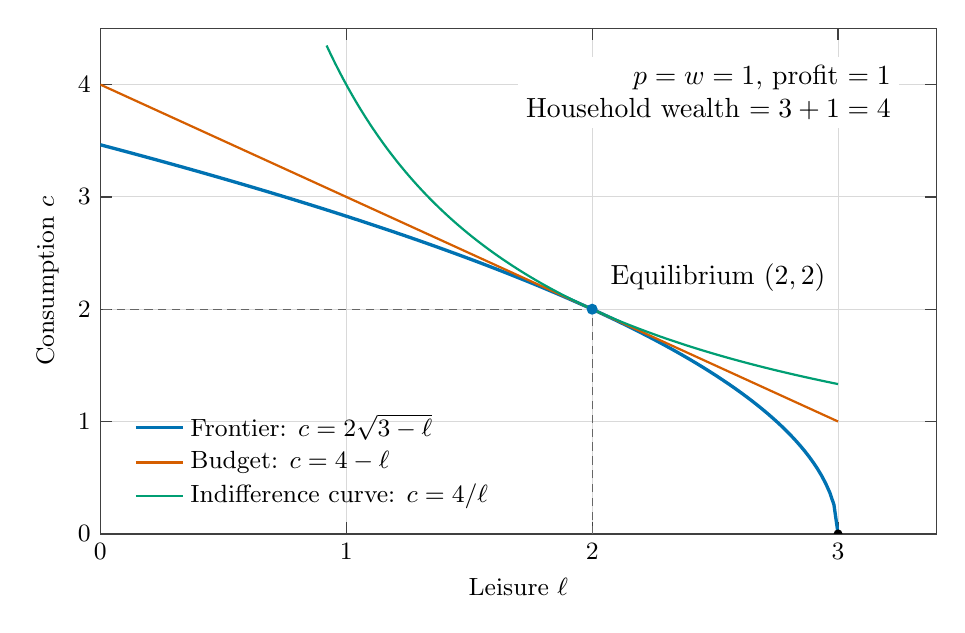
\begin{tikzpicture}
\begin{axis}[book axis,width=12.2cm,height=8cm,xmin=0,xmax=3.4,ymin=0,ymax=4.5,
 xlabel={Leisure $\ell$},ylabel={Consumption $c$},xtick={0,1,2,3},ytick={0,1,2,3,4},
 grid=major,legend style={at={(.03,.03)},anchor=south west}]
 \addplot[BookBlue,very thick,domain=0:3,samples=180]{2*sqrt(max(0,3-x))};
 \addlegendentry{Frontier: $c=2\sqrt{3-\ell}$}
 \addplot[BookOrange,thick,domain=0:3]{4-x};
 \addlegendentry{Budget: $c=4-\ell$}
 \addplot[BookGreen,thick,domain=.92:3,samples=120]{4/x};
 \addlegendentry{Indifference curve: $c=4/\ell$}
 \draw[BookGray,densely dashed] (axis cs:2,0)--(axis cs:2,2)--(axis cs:0,2);
 \fill[BookBlue] (axis cs:2,2) circle(2pt);
 \node[anchor=south west,fill=white,inner sep=2pt] at(axis cs:2.05,2.1){Equilibrium $(2,2)$};
 \fill (axis cs:3,0) circle(1.6pt);
 \node[anchor=north east,fill=white,inner sep=3pt,align=right] at(axis cs:3.25,4.25)
 {$p=w=1$, profit $=1$\\Household wealth $=3+1=4$};
\end{axis}
\end{tikzpicture}
\end{document}
